\subsection{Progettazione e Codifica Proof of Concept}
Questo periodo comincia al termine del periodo di Analisi preliminare e termina con la codifica
del Proof of Concept.\\
\begin{center}
\textbf{periodo:} dal 15-12-2022 al 11-01-2023\\
\end{center}
In questo periodo verranno completate le attività arretrate, per poi concentrarsi sulla 
progettazione e la codifica del Proof of Concept. Si andrà inoltre avanti con la stesura 
della documentazione. Questo periodo sarà suddiviso nelle attività trattate nella seguente sezione.
\subsubsection{Attività}
\begin{itemize}
\item \textbf{Glossario:} il documento viene costantemente aggiornato con nuovi termini;
\item \textbf{Piano di progetto:} viene aggiunta la pianificazione del periodo, il preventivo e il consultivo;  
\item \textbf{Analisi dei requisti:} si continua la stesura del documento, completando le attività arretrate dal periodo precedente;
\item \textbf{Piano di Qualifica:} documento nel quale vengono stabiliti gli obiettivi di qualità del prodotto;
\item \textbf{Norme di Progetto:} vengono aggiunte le norme relative alla scrittura del codice;
\item \textbf{Proof of Concept:} si realizza il Proof of Concept, una versione semplice, ma dimostrativa, del prodotto finale, per 
capire se è fattibile e darne una prova al proponente;   
\end{itemize}

\subsubsection{Periodi}
La fase di \textit{Progettazione e Codifica Proof of Concept} sarà suddivisa nei seguenti periodi:
\begin{itemize}
\item \textbf{Periodo 1:} \textit{dal 15-12-2022 al 21-12-2022}, Pianificazione del periodo corrente con relativo preventivo, completamento attività arretrate (stesura del documento di analisi dei requisiti).
\item \textbf{Periodo 2:} \textit{dal 22-12-2022 al 11-01-2023}, 
\end{itemize}

\subsubsection{Diagramma di Gantt fase Progettazione e Codifica Proof of Concept}
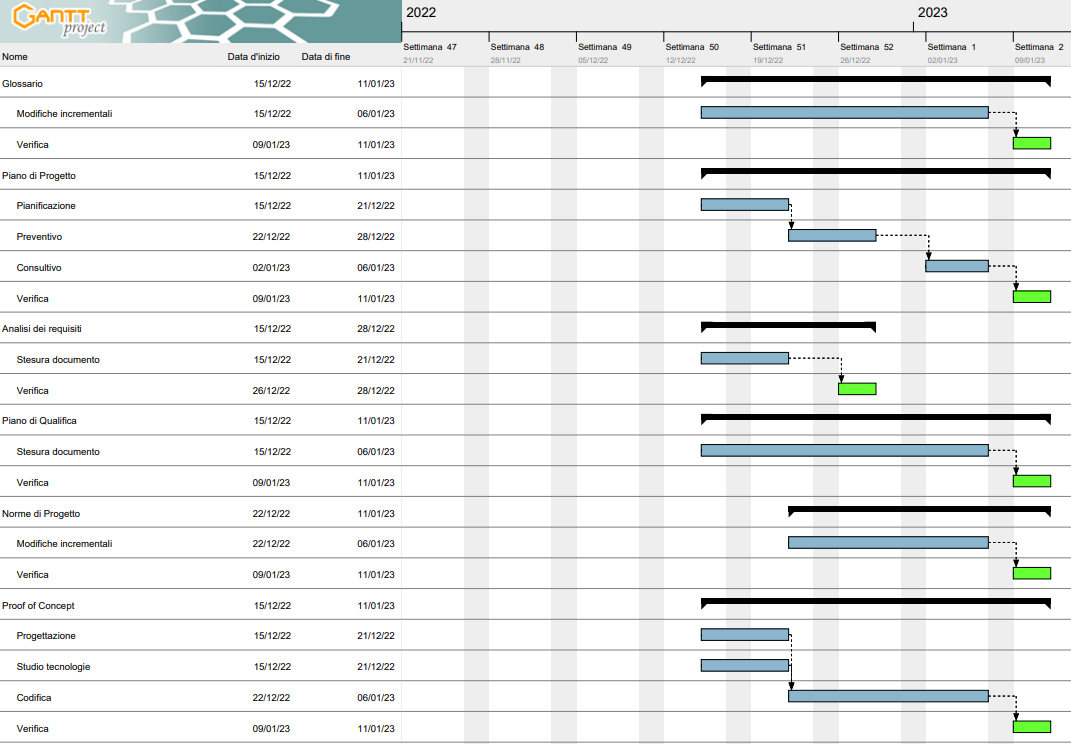
\includegraphics[scale=0.75]{image/gantt_secondo_periodo.png}
\captionof{figure}{Diagramma di Gantt fase di Progettazione e Codifica Proof of Concept}